%\newcommand{\F}{\mathbb{F}}
%\newcommand{\G}{\mathbb{G}}
\newcommand{\Cdel}{\ensuremath{c_{del}}}
\newcommand{\Cins}{\ensuremath{c_{ins}}}
\newcommand{\Cupd}{\ensuremath{c_{upd}}}
\renewcommand{\O}[1]{\ensuremath{\mathcal{O}(#1)}}

%indentation in code:
\algdef{SE}[SUBALG]{Indent}{EndIndent}{}{\algorithmicend\ }
\algtext*{Indent}
\algtext*{EndIndent}


\chapter{Tree-edit-distance algoritmus}

Jadro aplikacie lezi v pouziti tree-edit-distance (TED) algoritmu,
vdaka ktoremu dostaneme mapovanie medzi 2 RNA stromami. Mapovanie nam ukaze
spolocne casti oboch RNA stromov. TED algoritmus je obdoba Levenstheinoveho
string-edit-distance algoritmu. Problem u retazcov je specialnym pripadom
TED-u, kedy stromy zdegenerovali na cesty (spojovy zoznam).

\section{Hlavna myslienka TED-u}

Zaklad TED algoritmu je v rekurzivnom vzorci \ref{eq:ted} z \citet{DMRW} a \citet{RTED}. Vzdialenost medzi
lesmi F a G, $\delta(F, G)$ je definovana ako minimalny pocet editacnych operacii,
ktore z F urobia G. Pouzivame standardne editacne operacie - delete, insert, update.

\begin{figure}[H]
\centering
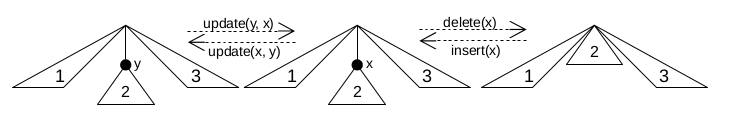
\includegraphics[width=140mm, height=30mm]{../img/TED_operations.png}
\caption{Ukazky TED operacii}
\label{obr:TED_operations}
\end{figure}

Delete, zmazanie vrcholu, znamena pripojit k predkovi vsetkych jeho potomkov so
zachovanim poradia medzi nimi. Insert, vlozenie vrcholu, je opacna operacia k
delete, co znamena, ze vkladame vrchol medzi rodica nejakych jeho, po sebe
nasledujucich potomkov. Update iba zmeni hodnotu vo vrchole stromu.

\section{Znacenie}

V tejto kapitole sa budeme riadit znacenim \citet{RTED}. Teda, pouzivame definiciu
stromu a lesa z \ref{def:strom}. Ak $F$ je les (strom), $N_F$ oznacuje mnozinu jeho vrcholov a $E_F$
mnozinu jeho hran. Plati dalej ze $E_F \subseteq N_F \times N_F$. $\emptyset$ oznacuje
prazdny strom, resp. prazdny les. Podles lesa $F$ je graf $\tilde{F}$ s vrcholmi
$N_{\tilde{F}} \subseteq N_F$ a hranami $E_{\tilde{F}} \subseteq E_F \cap N_{\tilde{F}} \times N_{\tilde{F}}$.
Obdobne to plati aj pre podstrom stromu $T$.
$F_{v}$ oznacuje podstrom $F$ zakoreneny vo $v$, t.j. v strome ostavaju iba potomkovia $v$.
$F - v$ budeme znacit les, ktory dostaneme zmazanim vrcholu $v$ z $F$, spolu so vsetkymi hranami
zasahujucimi do $v$. Podobne $F - F_{v}$ budeme znacit les, ktory dostaneme zmazanim podstromu
$F_{v}$ z $F$.

\begin{definice}[Editacna vzdialenost]
	Nech F a G su dva lesy. Editacna vzdialenost, tree-edit-distance - $\delta(F, G)$,
	medzi F a G je rovna minimalnej cene, za ktoru les F transformujeme na G.
\end{definice}

Vo vzorci \ref{eq:ted} pocitame editacnu vzdialenost $\delta(F, G)$,
\Cdel, \Cins a \Cupd su ceny zmazania, vlozenia a editacie vrcholu v strome
a $r_{F}$ a $r_{G}$ su korene, bud obidva najpravejsie alebo najlavejsie (tzn. vyberieme
najpravejsi/najlavejsi strom lesa a jeho koren).

\begin{figure}[H]\label{eq:ted}
\begin{subequations}
\begin{align}
	\begin{split}
	\delta(\emptyset, \emptyset) &=
		0
		\\
	\delta(F, \emptyset) &=
		\delta(F - r_{F}, \emptyset) + \Cdel(r_{F})
		\\
	\delta(\emptyset, G) &=
		\delta(\emptyset, G - r_{G}) + \Cins(r_{G})
	\end{split}
	\\[1ex]
	\delta(F, G) &=
		\begin{cases}
			\delta(F - r_{F}, G) + \Cdel(r_{F}) \\
			\delta(F, G - r_{G}) + \Cins(r_{G}) \\
			\delta(F - F_{r_{F}}, G - G_{r_{G}}) + \\
				\quad \delta(F_{r_{F}} - r_{F}, G_{r_{G}} - r_{G}) + \Cupd(r_{F}, r_{G})
		\end{cases}
\end{align}
\end{subequations}
\caption{Rekurzivny vzorec pre vypocet tree-edit-distance}
\end{figure}


\section{Algoritmy dynamickeho programovania}

\citet{TAI} predstavil algoritmus s priestorovou a casovou zlozitostou \O{m^3 \cdot n^3},
\citet{ZHANGSHASHA} algoritmus nasledne vylepsili pozorovanim toho, ze nepotrebujeme
vzdialenosti medzi vsetkymi parmi podlesov. Algoritmus mal casovu zlozitost \O{m^2 \cdot n^2}
a priestorovu \O{m \cdot n}. \citet{KLEIN} dosiahol casovu zlozitost \O{m^2 \cdot n \cdot \log{n}},
avsak jeho riesenie potrebovalo rovnako vela pamete.
\citet{DALUCQ} ukazali, ze minimalny cas na beh algoritmu je \O{m \cdot n \cdot \log{m} \cdot \log{n}}.
\citet{DMRW} predviedli worst-case optimalny algoritmus pre tree-edit-distance.
Jeho casova a priestorova zlozitost je \O{m^2 \cdot n \cdot (1 + \log{\frac{n}{m}})} a
\O{m \cdot n}. \citet{RTED} ukazali spojitost medzi efektivnostou predchadzajucich algoritmov
a tvarom stromov. Zovseobecnili predchadzajuce pristupy a vytvorili algoritmus beziaci
vo worst-case case \O{m^3} a priestore \O{m \cdot n}. Ich algoritmus je teda efektivny pre vsetky
tvary stromov a nikdy nespadne do worst-case, ak existuje lepsi smer vypoctu. 



\subsection{RTED: Robust Tree Edit Distance algoritmus}

Dalej sa v nasej praci budeme venovat vyhradne algoritmu RTED od tvorcov \citet{RTED}.
Ich algoritmus rozdelime na 2 casti, rovnako pomenovany RTED a GTED.

RTED (Robust Tree Edit Distance) algoritmus bude pre nas algoritmus na vypocet
optimalnej dekompozicnej strategie (viz definicia \ref{def:strategy})
a GTED (General Tree Edit Distance) algoritmus samotny vypocet rekurzie \ref{eq:ted}
s aplikovanim danej strategie.

\begin{definice}[Dekompozicna strategia]\label{def:strategy}
	Nech $F$ a $G$ su lesy. Dekompozicina strategia v rekurzii \ref{eq:ted} priradi
  kazdej dvojici podstromov $F_{v}$ a $G_{w}$ lesov $F$ a $G$ jednu cestu $\gamma_{T}$
  z korena do listu, kde $T \in \{F, G\}$.
	LRH dekompozicna strategia vybera vzdy najlavejsi/najpravejsi/najtazsi
	(left/right/heavy) vrchol na ceste z korena do listu. Najtazsi vrchol je taky
	v ktoreho podstrome je najviac vrcholov. 
\end{definice}

\begin{definice}
	Celkova dekompozicia lesa (full decomposition) $F$, $\mathcal{A}(F)$ je mnozina
	vsetkych podlesov F, ktore dostaneme rekurzivnym odstranenim najlavejsieho
	alebo najpravejsieho korenoveho vrcholu - $r_{R}(F)$ a $r_{L}(F)$ - z $F$
	a nasledne aj vsetkych jeho podlesov.
	\begin{align*}
		\mathcal{A}(\emptyset) &= \emptyset
		\\
		\mathcal{A}(F) &= {F} \cup \mathcal{A}(F - r_{L}(F)) \cup \mathcal{A}(F - r_{R}(F))
	\end{align*}
\end{definice}

\begin{figure}[H]
\centering
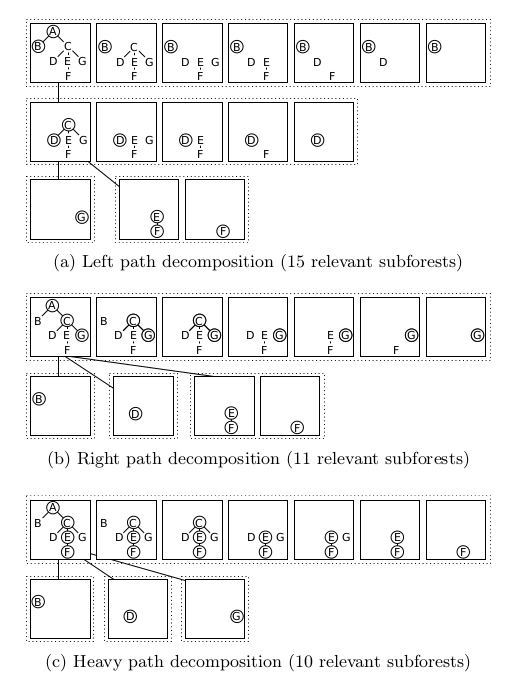
\includegraphics[width=85mm, height=100mm]{../img/LRH_decomposition.png}
%TODO vlastne obrazky
\caption{Celkova dekompozicia pomocou LRH strategii}
\label{obr:LRH_decomposition}
\end{figure}

\begin{definice}
	Relevant subtrees stromu $F$ pre root-leaf cestu $\gamma$ su definovane ako $F - \gamma$.
	Relevant subforests stromu $F$ pre nejaku root-leaf cestu $\gamma$ su definovane rekurzivne ako
	\begin{align*}
    \mathcal{F}(\emptyset, \gamma) &= \emptyset
		\\
		\mathcal{F}(F, \gamma) &= \{F\} \cup
		\begin{cases}
      \mathcal{F}(F - r_{R}(F), \gamma), \quad{} &\text{ak $r_{L}(F) \in \gamma$}
			\\
      \mathcal{F}(F - r_{L}(F), \gamma), &\text{v ostatnych pripadoch}
		\end{cases}
	\end{align*}
\end{definice}

Kazdy krok rekurzie \ref{eq:ted} je vypocitana v konstantnom case z inych podproblemov.
Doba behu zavisi na pocte podproblemov ktore potrebujeme vyratat, takze dekompozicna
strategia hraje velku ulohu v dobe behu algoritmu.

Ulohou RTEDu je najst strategiu s najnizsim poctom problemov, ktore potrebujeme vyratat,
zatial co ulohou GTEDu je podla danej strategie prejst celou rekurziou \ref{eq:ted} a vratit
vzdialenost medzi stromami $F$ a $G$.




\subsubsection{GTED: General Tree Edit Distance algoritmus}

Pozn. $D^{T}$ budeme oznacovat transponovanu maticu, teda
$D[F_{v}][G_{w}] = D^{T}[G_{w}][F_{v}]$, podobne $S^{T}$.

\begin{itemize}
  \item Vstup: Stromy $F$ a $G$, funkcia $S(F_{v}, G_{w}) = \gamma$
    na vypocet dekompozicnej strategie.
  \item Vystup: matica $D$ vzdialenosti medzi vsetkymi podstromami $F$ a $G$.
\end{itemize}

%TODO: napisat par teplych slov ako budu dane algoritmy fungovat, a az potom pridat detaily

\begin{algorithm}
  \caption{General Tree Edit Distance for LRH strategies}\label{alg:gted}
  \begin{algorithmic}[1]
    \Procedure {gted}{$F, G, D$}
      \State \Comment {Usporiadanie vrcholov je zlava doprava v postorder}
      \State \Comment {Plati, $id(root(F)) = \abs{F} - id(mostleft(F))$}
      \State $\gamma \gets S(F, G)$
      \If {$\gamma \in \gamma^{*}(F)$}
        \ForAll {$F' \in F - \gamma$}
          \State $D \gets D \cup \Call{gted}{F', G, D}$
        \EndFor
        \If {$\gamma = \gamma^{L}(F)$}
          \State $D \gets D \cup \Delta^{L}(F, G, \gamma, D)$
        \ElsIf {$\gamma = \gamma^{R}(F)$}
          \State $D \gets D \cup \Delta^{R}(F, G, \gamma, D)$
        \Else
          \State $D \gets D \cup \Delta^{H}(F, G, \gamma, D)$
        \EndIf
      \Else
      \State $D \gets D \cup (\Call{gted}{G, F, S^{T}, D^{T}})^{T}$
      \EndIf
      \State \Return {$D$}
    \EndProcedure
  \end{algorithmic}
\end{algorithm}

\begin{definice}[Single path function]\label{def:single_path_function}
  Oznacme $D$ maticu vzdialenosti medzi stromami $F_{v}$ a $G_{w}$,
  teda $D[F_{v}][G_{w}] = \delta(F_{v}, G_{w})$.
  Potom funkcia $\Delta(F, G, \gamma_{F}, D)$ ktora pocita vzdialenosti medzi podstromami
  stromov $F$ a $G$ pre root-leaf cestu $\gamma_{F}$ nazveme single-path funkciou.
\end{definice}

Nasledovat budu 2 algoritmy na vypocet single-path-function, algoritmus \ref{alg:ZHANGSHASHA}
je z dielne \citet{ZHANGSHASHA} a algoritmus \ref{alg:DMRW} je od \citet{DMRW}.


\begin{algorithm}
  \caption{Zhang \& Shasha: Single path function}
  \label{alg:ZHANGSHASHA}
  \begin{algorithmic}[1]
    \Procedure {$\Delta^{L}$}{$F, G, \gamma, D$}
      \State $L_{F} \gets id(mostleft(F))$
      \State $L_{G} \gets id(mostleft(G))$
      \State $R_{F} \gets id(root(F))$
      \State $R_{G} \gets id(root(G))$

      \State $forestdistance \gets$ pole indexovane podlesmi stromov $F$ a $G$
      \State $forestdistance[\emptyset, \emptyset] := 0$
      \For {$i := L_{F}$ to $R_{F}$}
        \State $forestdistance[F[L_{F} \dotsc i], \emptyset] :=$
        \Indent
          \State $forestdistance[L_{F} \dotsc i$ - $1] + C_{del}(F[i])$
        \EndIndent
      \EndFor

      \For {$j := L_{G}$ to $R_{G}$}
        \State $forestdistance[\emptyset, G[L_{G} \dotsc j]] :=$
        \Indent
          \State $forestdistance[\emptyset, G[L_{G} \dotsc j$ - $1]] + C_{ins}(G[j])$
        \EndIndent
      \EndFor

      \For {$i := L_{F}$ to $R_{F}$}
        \For {$j := L_{G}$ to $R_{G}$}
          \If {both subtrees $F[L_{F} \dotsc i] \land G[L_{G} \dotsc j]$ are trees}
            \State $C_{min} := min \{$
            \Indent
              \State $forestdistance(F[L_{F} \dotsc i$ - $1], G[L_{G} \dotsc j] + C_{del}(F[i])$,
              \State $forestdistance(F[L_{F} \dotsc i], G[L_{G} \dotsc j$ - $1] + C_{ins}(G[j])$,
              \State $forestdistance(F[L_{F} \dotsc i$ - $1], G[L_{G} \dotsc j$ - $1] +$
              \Indent
                \State $C_{upd}(F[i], G[j]) \}$
              \EndIndent
            \EndIndent
            \State $forestdistance[F[L_{F} \dotsc i], G[L_{G} \dotsc j]] := C_{min}$
            \State $D[i, j] := C_{min}$
          \Else
            \State $C_{min} := min \{$
            \Indent
              \State $forestdistance(F[L_{F} \dotsc i$ - $1], G[L_{G} \dotsc j] + C_{del}(F[i])$,
              \State $forestdistance(F[L_{F} \dotsc i], G[L_{G} \dotsc j$ - $1] + C_{ins}(G[j])$,
              \State $forestdistance(F[L_{F} \dotsc id(mostleft(F[i]))$ - $1]$,
              \Indent
                \State $G[L_{G} \dotsc id(mostleft(G[j]))$ - $1] + D[i, j] \}$
              \EndIndent
            \EndIndent
            \State $forestdistance[F[L_{F} \dotsc i], G[L_{G} \dotsc j]] := C_{min}$
          \EndIf
        \EndFor
      \EndFor
    \EndProcedure
  \end{algorithmic}
\end{algorithm}

\begin{algorithm}
  \caption{DMRW}
  \label{alg:DMRW}
  %TODO
\end{algorithm}




